\chapter{Identificação e Análise de Oportunidades Tecnológicas e Territoriais}
\label{cap:08}
\markboth{CAPÍTULO 8: ANÁLISE DE OPORTUNIDADES}{CAPÍTULO 8: ANÁLISE DE OPORTUNIDADES}

\noindent\tagQuant\ \tagTerritorio

\begin{capObjetivos}
  Ao concluir este capítulo, você será capaz de:
  \begin{enumerate}[leftmargin=1.5em, itemsep=2pt]
    \item Distinguir a Teoria da Descoberta da Teoria da Criação de Oportunidades (\textit{Alvarez \& Barney, 2007}) e suas implicações para a estratégia empresarial.
    \item Identificar sinais territoriais de oportunidade a partir das sete fontes de inovação sistematizadas por Peter Drucker (1985).
    \item Calcular e cruzar o dimensionamento de mercado \textbf{TAM, SAM e SOM} pelas abordagens \textit{top-down} e \textit{bottom-up}.
    \item Avaliar instrumentos de \textbf{Propriedade Intelectual (PI)}, patentes, modelos de utilidade, registro de software, cultivares, marcas e segredo industrial, e a função da busca de anterioridade.
  \end{enumerate}
\end{capObjetivos}

\begin{capRevisao}
  Retome três noções essenciais dos capítulos anteriores:
  \begin{itemize}[leftmargin=1.5em, itemsep=2pt]
    \item \textbf{Nexo Indivíduo–Oportunidade:} a identificação de oportunidades depende tanto das assimetrias do mercado quanto do conhecimento prévio acumulado pelo agente.
    \item \textbf{Incerteza vs. Risco:} oportunidades em mercados conhecidos permitem estimativas probabilísticas; oportunidades em mercados inéditos requerem construção iterativa.
    \item \textbf{Indicações Geográficas (IGs) e Ativos Territoriais:} conforme visto na Unidade I, ativos específicos de um território (saberes, biodiversidade, cadeias produtivas) podem gerar diferenciação não replicável.
  \end{itemize}
\end{capRevisao}

\etapa{3}{Explicação Teórica, Vocabulário Prévio e Modelos}

\begin{boxSimbolo}[Vocabulário Conceitual e Símbolos do Capítulo 8]
  \begin{tabularx}{\textwidth}{@{}l >{\raggedright\arraybackslash}X@{}}
    \textbf{TAM} & \textit{Total Addressable Market}: demanda total máxima global ou nacional para uma categoria de solução. \\
    \textbf{SAM} & \textit{Serviceable Available Market}: parcela do TAM alcançável pelo modelo de negócio, restrições geográficas e recorte regulatório. \\
    \textbf{SOM} & \textit{Serviceable Obtainable Market}: parcela realista do SAM que o empreendimento consegue capturar no horizonte de 3 a 5 anos dada sua capacidade produtiva e comercial. \\
    \textbf{PI / INPI} & Propriedade Intelectual e Instituto Nacional da Propriedade Industrial. \\
    \textbf{PI vs. MU} & Patente de Invenção (vigência de 20 anos) e Modelo de Utilidade (vigência de 15 anos). \\
    \textbf{FTO} & \textit{Freedom to Operate}: análise que verifica se uma tecnologia pode ser comercializada sem infringir patentes vigentes de terceiros. \\
  \end{tabularx}
\end{boxSimbolo}

\section{Teoria da Descoberta vs. Teoria da Criação (Alvarez \& Barney, 2007)}

Uma questão central na estratégia empreendedora indaga se as oportunidades existem objetivamente no ambiente econômico aguardando quem as encontre, ou se são construídas pelas ações dos próprios empreendedores. Sharon Alvarez e Jay Barney (2007) organizaram esse debate em duas teorias complementares.

Na \textbf{Teoria da Descoberta}, as oportunidades existem de forma independente dos empreendedores, originadas por choques exógenos como novas descobertas científicas, mudanças demográficas, alterações regulatórias ou falhas de mercado. O contexto decisório é de \textbf{risco}: é possível coletar dados, estimar o tamanho da demanda e formular planos baseados em lógica \textit{Causation}. O empreendedor diferencia-se pela atenção alerta (\textit{alertness}) para enxergar lacunas antes dos concorrentes.

Na \textbf{Teoria da Criação}, as oportunidades emergem de forma endógena à medida que empreendedores interagem com clientes, fornecedores e instituições, testando hipóteses e modificando preferências. O contexto decisório é de \textbf{incerteza knightiana}, pois inexistem dados prévios confiáveis para pesquisa de mercado tradicional. Nesse cenário, prevalece a lógica \textit{Effectuation}, na qual o aprendizado iterativo molda simultaneamente o produto e o mercado.

\begin{center}
\renewcommand{\arraystretch}{1.22}
\small
\begin{tabularx}{\textwidth}{@{}l >{\raggedright\arraybackslash}X >{\raggedright\arraybackslash}X@{}}
  \toprule
  \rowcolor{etIndigo}
  \textcolor{white}{\bfseries Critério} & \textcolor{white}{\bfseries Teoria da Descoberta} & \textcolor{white}{\bfseries Teoria da Criação} \\
  \midrule
  Natureza da oportunidade & Objetiva, gerada por choques exógenos. & Endógena, construída na ação social e técnica. \\
  \rowcolor{bgGray}
  Condição de informação & Risco mensurável por dados históricos. & Incerteza radical sem série histórica. \\
  Estratégia recomendada & Planejamento preditivo (\textit{Causation}). & Experimentação iterativa (\textit{Effectuation}). \\
  \rowcolor{bgGray}
  Exemplo territorial & Software para atender nova exigência fiscal agrícola. & Criação de mercado para créditos de biodiversidade da Caatinga. \\
  \bottomrule
\end{tabularx}
\end{center}

\section{As 7 Fontes de Inovação de Drucker (1985) e Sinais Territoriais}

Para sistematizar a observação de oportunidades sem depender de inspiração aleatória, Peter Drucker (1985) identificou sete fontes de oportunidade inovadora, divididas entre quatro fontes internas ao setor produtivo e três fontes externas situadas no ambiente social e intelectual. No planejamento territorial, as quatro primeiras emergem diretamente da dinâmica das cadeias produtivas locais. O \textbf{inesperado} manifesta-se em sucessos ou fracassos imprevistos de produtos regionais, como ocorre quando um subproduto descartado na agroindústria passa a atrair procura cosmética. A \textbf{incongruência} revela o descompasso entre a realidade econômica de um território e as premissas vigentes, visível em regiões com elevada produção primária e baixíssima agregação de valor local. De modo complementar, a \textbf{necessidade de processo} aponta gargalos técnicos específicos que travam o rendimento regional, a exemplo da elevada perda pós-colheita decorrente da falta de pré-resfriamento móvel, enquanto as \textbf{mudanças na estrutura da indústria ou do mercado} abrem brechas por meio da descentralização logística, da transição energética ou da abertura de compras públicas sustentáveis.

As três fontes externas ampliam esse diagnóstico ao captar transformações demográficas, culturais e científicas que reconfiguram a demanda territorial. As \textbf{mudanças demográficas} abrangem o envelhecimento da população rural, o êxodo ou o retorno de jovens qualificados pela interiorização do ensino superior, alterando a disponibilidade de mão de obra e o perfil de consumo. Já as \textbf{mudanças de percepção} refletem a valorização crescente de rastreabilidade, agroecologia, economia circular e origem territorial certificada por parte dos compradores. Integrando esse conjunto, o \textbf{novo conhecimento} decorre de avanços científicos em biotecnologia, sensoriamento remoto, novos materiais ou inteligência artificial passíveis de adaptação a problemas locais concretos.

\section{Dimensionamento de Mercado: TAM, SAM e SOM}

Identificar uma necessidade real exige quantificar a escala econômica da oportunidade antes de imobilizar capital. O funil \textbf{TAM–SAM–SOM} evita projeções infladas, como reivindicar um percentual arbitrário de um mercado bilionário, e conecta a ambição estratégica à capacidade operacional efetiva da equipe. Conforme ilustra a Figura~\ref{fig:08_tam_sam_som}, o dimensionamento parte da demanda máxima teórica (TAM), aplica filtros geográficos e regulatórios para delimitar o mercado alcançável (SAM) e converge para a fatia realista obtenível (SOM) no horizonte inicial de operação.

\begin{figure}[H]
  \centering
  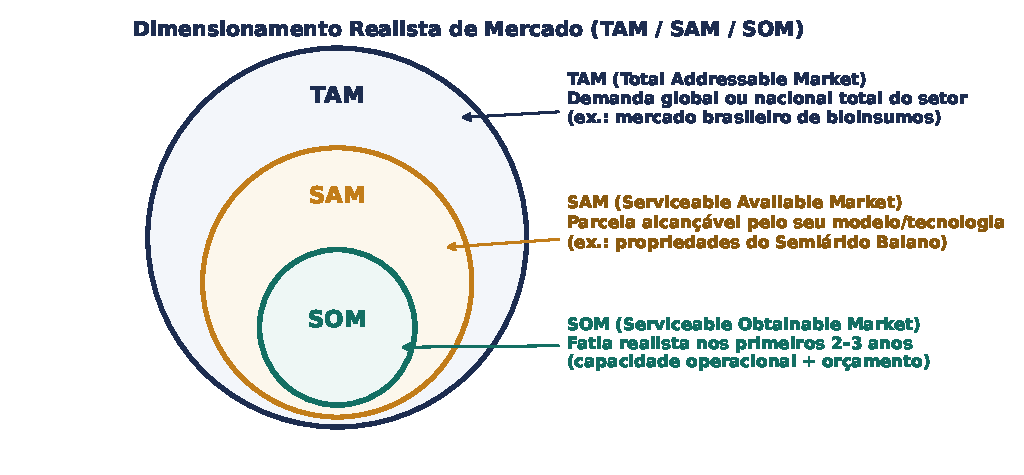
\includegraphics[width=0.90\textwidth]{figures/fig08_tam_sam_som.pdf}
  \caption{Funil de dimensionamento de mercado TAM, SAM e SOM articulando estimativas \textit{top-down} e \textit{bottom-up}.}
  \label{fig:08_tam_sam_som}
\end{figure}

\begin{boxFormula}[Modelagem Quantitativa TAM, SAM e SOM (\textit{Top-Down} e \textit{Bottom-Up})]
  \textbf{1. Abordagem \textit{Top-Down} (de cima para baixo):} parte de dados macroeconômicos ou setoriais agregados e aplica filtros sucessivos de segmentação geográfica e técnica.
  \[
    \text{TAM} = N_{\text{total}} \times T_{\text{anual}}, \qquad
    \text{SAM} = \text{TAM} \times f_{\text{geo}} \times f_{\text{seg}}, \qquad
    \text{SOM}_{\text{TD}} = \text{SAM} \times s_{\text{cap}},
  \]
  onde $N_{\text{total}}$ é o universo potencial de clientes no mercado amplo, $T_{\text{anual}}$ é o gasto médio anual por cliente, $f_{\text{geo}}$ e $f_{\text{seg}}$ são os fatores de recorte geográfico e de aderência ao modelo de negócio, e $s_{\text{cap}}$ é a fatia de mercado (\textit{market share}) realista no horizonte planejado.

  \vspace{4pt}
  \textbf{2. Abordagem \textit{Bottom-Up} (de baixo para cima):} constrói o SOM a partir da capacidade operacional efetiva da equipe, da produção ou dos canais de venda:
  \[
    \text{SOM}_{\text{BU}} = \min\bigl(C_{\text{máx}}, \; N_{\text{alvo}} \times Q_{\text{anual}}\bigr) \times P_{\text{unitário}},
  \]
  onde $C_{\text{máx}}$ é a capacidade máxima anual de entrega ou atendimento, $N_{\text{alvo}}$ é o número de clientes alcançáveis pela força comercial, $Q_{\text{anual}}$ é o volume médio anual por cliente e $P_{\text{unitário}}$ é o preço unitário. A consistência do plano exige verificar se $\text{SOM}_{\text{BU}} \le \text{SAM}$.
\end{boxFormula}

\section{Propriedade Intelectual (PI) na Avaliação de Oportunidades}

Em empreendimentos de base tecnológica, a apropriação dos retornos da inovação depende da estratégia de \textbf{Propriedade Intelectual (PI)}. No Brasil, a proteção industrial é regida principalmente pela Lei nº 9.279/1996 (Lei da Propriedade Industrial), pela Lei nº 9.609/1998 (Software) e pela Lei nº 9.456/1997 (Cultivares). A escolha do ativo de PI equilibra custo, tempo de concessão e risco de engenharia reversa entre diferentes regimes jurídicos. Para invenções técnicas, a \textbf{Patente de Invenção (PI)} protege produtos ou processos inéditos com atividade inventiva e aplicação industrial por 20 anos a partir do depósito, exigindo divulgação pública integral do método no documento patentário, ao passo que o \textbf{Modelo de Utilidade (MU)} resguarda por 15 anos objetos de uso prático com nova forma ou disposição que resulte em melhoria funcional no uso ou fabricação. No domínio digital e biológico, o \textbf{Registro de Programa de Computador (Software)} protege o código-fonte como direito autoral no INPI por 50 anos a partir de 1º de janeiro do ano subsequente à publicação ou criação, enquanto a \textbf{Proteção de Cultivares} junto ao SNPC/MAPA aplica-se a novas variedades vegetais desenvolvidas por melhoramento genético, sendo vital para a bioeconomia regional.

Quando a vantagem competitiva reside na identidade comercial, na origem ou no sigilo de processo, outros instrumentos tornam-se prioritários. As \textbf{Marcas} protegem sinais distintivos por 10 anos renováveis, e as \textbf{Indicações Geográficas (IGs)} vinculam reputação ou qualidade ao território por meio de Indicação de Procedência ou Denominação de Origem. Em contraposição ao registro público, o \textbf{Segredo Industrial} mantém sigilo sobre formulações, parâmetros de processo ou algoritmos internos sem prazo legal de expiração, desde que esses elementos resistam à descoberta por engenharia reversa.

Antes de investir em P\&D ou lançar um produto, é obrigatório realizar a \textbf{busca de anterioridade} em bases públicas (INPI, Espacenet, PATENTSCOPE, Google Patents). Essa busca cumpre duas funções complementares, evitando o desperdício de recursos ao reinventar soluções já existentes no estado da técnica e verificando a \textbf{liberdade de operação (\textit{Freedom to Operate}, FTO)} para assegurar que a comercialização não violará patentes vigentes no território de venda.

\etapa{4}{Estudos de Caso e Exemplos Resolvidos em 7 Passos}

\begin{boxExemplo}{8.1}{Dimensionamento \textit{Top-Down}: Plataforma de Rastreabilidade do Mel}
  \passoEnunciado{Uma startup baiana desenvolve uma plataforma digital de rastreabilidade sanitária e certificação de origem para cooperativas e produtores de mel do Semiárido.}
  \passoDados{Universo nacional estimado de apicultores formais e associados: $N_{\text{total}} = 120.000$ produtores. Assinatura anual da plataforma: $T_{\text{anual}} = \text{R\$\,1.800,00/ano}$. Recorte geográfico e de perfil cooperativado no Nordeste: $f_{\text{geo}} \times f_{\text{seg}} = 25\%$ ($0{,}25$). Meta realista de captura em 3 anos com equipe de 3 consultores territoriais: $s_{\text{cap}} = 4\%$ ($0{,}04$) do SAM.}
  \passoPedido{Calcular o TAM, o SAM e o SOM anual pela abordagem \textit{top-down}, além do número de apicultores pagantes necessários para atingir o SOM.}
  \passoMetodo{Aplicação sequencial das equações \textit{top-down} de TAM, SAM e SOM.}
  \passoContas{
    \[
      \text{TAM} = 120.000 \times 1.800 = \text{R\$\,216.000.000,00/ano}.
    \]
    Aplicando o fator de recorte regional e de aderência ($0{,}25$):
    \[
      \text{SAM} = 216.000.000 \times 0{,}25 = \text{R\$\,54.000.000,00/ano} \quad (30.000\text{ apicultores}).
    \]
    Aplicando a meta de captura ($4\%$ do SAM):
    \[
      \text{SOM}_{\text{TD}} = 54.000.000 \times 0{,}04 = \text{R\$\,2.160.000,00/ano}.
    \]
    O número de apicultores pagantes no SOM é $30.000 \times 0{,}04 = 1.200$ produtores (400 produtores atendidos por consultor).
  }
  \passoResposta{$\text{TAM} = \text{R\$\,216,0 milhões/ano}$; $\text{SAM} = \text{R\$\,54,0 milhões/ano}$; $\text{SOM} = \text{R\$\,2,16 milhões/ano}$ (1.200 produtores).}
  \passoVerificacao{Atender 1.200 apicultores por meio de cooperativas regionais com 3 consultores (cerca de 15 a 20 cooperativas de 60 a 80 associados cada) é operacionalmente factível no horizonte de 3 anos.}
\end{boxExemplo}

\begin{boxExemplo}{8.2}{Dimensionamento \textit{Bottom-Up}: Bioinsumo para Cacauicultura no Sul da Bahia}
  \passoEnunciado{Uma biofábrica emergente no Sul da Bahia produz um biofungicida à base de \textit{Trichoderma} para controle da vassoura-de-bruxa e podridão-parda em lavouras de cacau.}
  \passoDados{Capacidade máxima da biofábrica piloto: $C_{\text{máx}} = 48.000\text{ litros/ano}$. Dose recomendada: $8\text{ litros/ha/ano}$. Área média de cacau por propriedade atendida: $15\text{ ha}$. Preço unitário: $P_{\text{unitário}} = \text{R\$\,45,00/litro}$. Área regional de cacau tecnificado (SAM físico): $180.000\text{ ha}$.}
  \passoPedido{Calcular o SOM anual pela abordagem \textit{bottom-up}, o número máximo de hectares e propriedades atendidas, o SAM financeiro regional e a fatia do SAM representada pelo SOM.}
  \passoMetodo{Cálculo da restrição produtiva \textit{bottom-up} e comparação com o SAM regional.}
  \passoContas{
    Como a capacidade é de $48.000\text{ L/ano}$ e o preço é R\$\,45,00/L, o SOM limitado pela capacidade produtiva é:
    \[
      \text{SOM}_{\text{BU}} = 48.000 \times 45{,}00 = \text{R\$\,2.160.000,00/ano}.
    \]
    Hectares atendidos: $48.000 / 8 = 6.000\text{ ha/ano}$. Propriedades atendidas: $6.000 / 15 = 400\text{ propriedades/ano}$.
    O gasto anual por hectare é $8 \times 45{,}00 = \text{R\$\,360,00/ha}$. Assim, o SAM regional é:
    \[
      \text{SAM} = 180.000 \times 360{,}00 = \text{R\$\,64.800.000,00/ano}.
    \]
    A participação do SOM no SAM é:
    \[
      s_{\text{cap}} = \frac{2.160.000}{64.800.000} = 0{,}0333 = 3{,}33\%.
    \]
  }
  \passoResposta{$\text{SOM}_{\text{BU}} = \text{R\$\,2,16 milhões/ano}$ (6.000 ha; 400 propriedades), equivalente a 3{,}33\% do SAM regional de R\$\,64,80 milhões/ano.}
  \passoVerificacao{O cruzamento \textit{bottom-up} confirma que a restrição inicial está na capacidade da biofábrica e não na falta de área agrícola disponível.}
\end{boxExemplo}

\begin{boxExemplo}{8.3}{Diagnóstico de Oportunidade por Descoberta vs. Criação}
  \passoEnunciado{Uma equipe técnica compara duas propostas de negócio no Semiárido: (A) dispositivo acústico para detectar vazamentos em adutoras rurais já operadas por companhias de saneamento; (B) plataforma para comercializar créditos de conservação da biodiversidade da Caatinga para empresas globais.}
  \passoDados{Proposta A: existem 14.000 km de adutoras com índice médio de perda física de 38\% e orçamento anual conhecido de manutenção. Proposta B: não há marco regulatório consolidado nem padrão de precificação aceito por compradores para créditos de biodiversidade da Caatinga.}
  \passoPedido{Classificar cada proposta segundo Alvarez e Barney (2007) e definir o método de validação apropriado para cada caso.}
  \passoMetodo{Mapeamento epistemológico entre condição de risco/incerteza e teoria da oportunidade.}
  \passoContas{
    Na Proposta A, o problema (perda de 38\% em 14.000 km de rede) e o pagador existem objetivamente; a oportunidade é de \textbf{Descoberta}, permitindo calcular economia potencial de água e estruturar licitação ou venda técnica (\textit{Causation}). Na Proposta B, tanto a métrica do ativo quanto a disposição a pagar precisam ser negociadas e legitimadas com compradores-piloto e certificadoras; trata-se de oportunidade de \textbf{Criação}, exigindo prototipagem de contratos e alianças (\textit{Effectuation}).
  }
  \passoResposta{Proposta A corresponde à Teoria da Descoberta (risco mensurável, abordagem \textit{Causation}); Proposta B corresponde à Teoria da Criação (incerteza radical, abordagem \textit{Effectuation}).}
  \passoVerificacao{Tratar a Proposta B com pesquisa de mercado estatística tradicional produziria projeções irreais, pois o mercado ainda não está constituído.}
\end{boxExemplo}

\begin{boxExemplo}{8.4}{Leitura de Sinais Territoriais pelas 7 Fontes de Drucker}
  \passoEnunciado{No Recôncavo Baiano, observa-se forte crescimento da produção de mandioca por agricultores familiares, acompanhado de elevada perda de qualidade da farinha por secagem artesanal irregular em períodos chuvosos e aumento da demanda urbana por produtos sem glúten rastreados.}
  \passoDados{Perda atual por umidade excessiva: 18\% da produção nas safras de outono. Preço da farinha comum a granel: R\$\,4,50/kg. Preço da farinha embalada com certificação de origem e padrão granulométrico: R\$\,11,00/kg.}
  \passoPedido{Identificar quais fontes de Drucker (1985) estão presentes e calcular o ganho bruto de valor por tonelada processada ao migrar para o segmento diferenciado.}
  \passoMetodo{Mapeamento das sete fontes de inovação e cálculo de agregação de valor unitária.}
  \passoContas{
    Fontes presentes: \textbf{necessidade de processo} (secagem irregular gerando perda de 18\%) e \textbf{mudança de percepção} (busca urbana por alimentos sem glúten e rastreabilidade).
    Para 1.000 kg de produto base:
    \[
      \text{Receita comum (com perda de 18\%)} = 820\text{ kg} \times 4{,}50 = \text{R\$\,3.690,00}.
    \]
    Com secador solar híbrido que reduz a perda para 3\% e habilita embalagem certificada:
    \[
      \text{Receita diferenciada} = 970\text{ kg} \times 11{,}00 = \text{R\$\,10.670,00}.
    \]
    Ganho bruto adicional por lote de 1.000 kg iniciais: $10.670,00 - 3.690,00 = \text{R\$\,6.980,00}$ ($+189{,}16\%$).
  }
  \passoResposta{As fontes são necessidade de processo e mudança de percepção, gerando potencial de ganho bruto adicional de R\$\,6.980,00 por tonelada base processada.}
  \passoVerificacao{A análise deve ser complementada na modelagem de custos pelo CAPEX e OPEX do secador e da embalagem, tema da Unidade III.}
\end{boxExemplo}

\begin{boxExemplo}{8.5}{Estratégia de Propriedade Intelectual e Busca de Anterioridade}
  \passoEnunciado{Uma equipe desenvolveu um secador solar híbrido de frutas composto por: (i) novo arranjo mecânico de bandejas dobráveis de baixo custo; (ii) controlador eletrônico com algoritmo proprietário de ajuste térmico; e (iii) marca comercial para vender frutas desidratadas.}
  \passoDados{A busca de anterioridade no INPI e na base Espacenet não encontrou o arranjo mecânico específico das bandejas, mas identificou uma patente estrangeira vigente no Brasil sobre o circuito eletrônico básico de controle PWM utilizado.}
  \passoPedido{Definir o portfólio adequado de proteção de PI para os três ativos e indicar a implicação da patente estrangeira identificada na busca de FTO.}
  \passoMetodo{Adequação entre natureza do ativo tecnológico, regime jurídico de PI e análise de liberdade de operação (FTO).}
  \passoContas{
    (i) O arranjo mecânico de bandejas que melhora a ergonomia e eficiência de uso sem ruptura científica radical enquadra-se em \textbf{Modelo de Utilidade (MU)} (15 anos); (ii) o algoritmo embarcado pode ser protegido por \textbf{Registro de Software} (código-fonte) e \textbf{Segredo Industrial} (parâmetros de calibração térmica); (iii) a identidade comercial recebe proteção via \textbf{Registro de Marca} no INPI. Quanto à patente estrangeira vigente no Brasil para o circuito PWM, há risco de infração na análise de FTO: a startup deve substituir o circuito por componente comercial licenciado de prateleira ou redesenhar o estágio de potência (\textit{design around}).
  }
  \passoResposta{Portfólio recomendado: MU (bandejas) + Registro de Software/Segredo Industrial (algoritmo) + Marca (nome comercial), com substituição do circuito PWM patenteado para garantir FTO.}
  \passoVerificacao{A busca de anterioridade prévia evitou que a startup investisse em hardware sujeito a bloqueio judicial por infração de patente.}
\end{boxExemplo}

\etapa{5}{Armadilhas Conceituais e Erros Mais Comuns}

\begin{boxErro}[Erro 1: Confundir TAM com Receita Alcançável (\textit{Top-Down} Ingênuo)]
  Declarar em um projeto que ``se capturarmos apenas 1\% de um mercado nacional de R\$\,10 bilhões, faturaremos R\$\,100 milhões'' é uma falácia clássica. Sem explicitar os canais de venda, a força comercial e a capacidade produtiva (\textit{bottom-up}), esse número não possui sustentação operacional.
\end{boxErro}

\begin{boxErro}[Erro 2: Patentear Tudo Indiscriminadamente Sem Analisar Engenharia Reversa]
  Depositar uma patente de invenção exige divulgar integralmente o modo de fazer a tecnologia e arcar com taxas e anuidades por até 20 anos. Se o diferencial reside em um parâmetro de processo ou formulação interna difícil de detectar no produto final, o segredo industrial pode proteger melhor do que a patente pública.
\end{boxErro}

\begin{boxErro}[Erro 3: Ignorar a Territorialidade das Patentes na Busca de Anterioridade]
  Acreditar que uma patente concedida apenas nos Estados Unidos ou na Europa impede a produção no Brasil, ou, inversamente, assumir que uma tecnologia disponível em artigo acadêmico tem liberdade de operação comercial, leva a decisões jurídicas equivocadas. Patentes têm validade territorial nacional.
\end{boxErro}

\begin{boxErro}[Erro 4: Tratar Oportunidade de Criação como Se Fosse de Descoberta]
  Aplicar questionários de intenção de compra para produtos totalmente inéditos gera falsos positivos ou rejeições por incompreensão. Quando o mercado ainda está sendo criado, a validação requer protótipos reais e experimentos de uso, não pesquisas declaratórias abstratas.
\end{boxErro}

\etapa{6}{Lista de Exercícios (15 Questões em 3 Níveis)}

\textbf{Nível 1, Fundamentos Conceituais (Questões 1 a 5)}

\begin{enumerate}[leftmargin=1.5em, itemsep=6pt]
  \item Explique a diferença central entre a Teoria da Descoberta e a Teoria da Criação de oportunidades (Alvarez \& Barney, 2007) quanto ao papel da ação empreendedora e ao nível de incerteza.
  \espacoResolucao[1.8cm]

  \item Escolha três das sete fontes de inovação de Drucker (1985) e dê um exemplo concreto de sinal territorial no estado da Bahia para cada uma delas.
  \espacoResolucao[1.8cm]

  \item Defina TAM, SAM e SOM e explique por que as abordagens \textit{top-down} e \textit{bottom-up} devem ser cruzadas para validar um plano de negócios.
  \espacoResolucao[1.8cm]

  \item Compare Patente de Invenção, Modelo de Utilidade e Segredo Industrial quanto ao objeto protegido, ao prazo de vigência e à exigência de divulgação pública.
  \espacoResolucao[1.8cm]

  \item O que significa \textit{Freedom to Operate} (FTO) e por que sua análise difere da verificação de novidade para depósito de patente?
  \espacoResolucao[1.8cm]

  \item \textbf{(Nível 2, Aplicações Numéricas)} Um mercado nacional conta com $80.000$ pequenas indústrias de alimentos que gastam em média R\$\,3.000,00/ano em controle de qualidade laboratorial. O segmento regional aderente a um kit portátil rápido corresponde a 20\% desse universo. A startup estima capturar 5\% desse mercado regional em 4 anos. Calcule o TAM, o SAM e o SOM \textit{top-down}.
  \espacoResolucao[2.3cm]

  \item Considerando o exercício anterior, suponha que a startup disponha de capacidade inicial de montagem de apenas $600\text{ kits/ano}$ vendidos a R\$\,3.000,00 cada. Calcule o SOM \textit{bottom-up} e compare-o com o SOM \textit{top-down} obtido. Há gargalo produtivo ou comercial?
  \espacoResolucao[2.3cm]

  \item Uma cooperativa de agricultura familiar possui 250 associados com área média de 4 hectares de mandioca cada. Uma solução de bioestimulante custa R\$\,120,00/hectare/ano. Se a meta de adesão inicial na cooperativa for de 60\% dos associados no Ano 1, qual será o SOM \textit{bottom-up} dessa carteira?
  \espacoResolucao[2.2cm]

  \item O mercado endereçável disponível (SAM) para sensores de monitoramento hídrico em municípios do Semiárido é de 1.100 municípios, com receita anual média de R\$\,18.000,00/município. Uma startup projeta faturamento de R\$\,1.980.000,00 no Ano 3. Qual percentual do SAM esse faturamento representa e quantos municípios precisam ser contratados?
  \espacoResolucao[2.2cm]

  \item Uma empresa comercializa farinha de licuri a granel com perda de 15\% na armazenagem (preço de R\$\,16,00/kg). Ao adotar embalagem a vácuo com marca registrada, a perda cai para 2\% e o preço sobe para R\$\,25,00/kg. Para um lote bruto inicial de 500 kg, qual o aumento percentual de receita?
  \espacoResolucao[2.3cm]

  \item \textbf{(Nível 3, Análise Territorial e Estratégica)} Uma equipe de pesquisa desenvolveu uma nova variedade de palma forrageira resistente à cochonilha-do-carmim e um software de manejo hídrico associado. Indique os regimes jurídicos de PI adequados para cada ativo no Brasil e justifique.
  \espacoResolucao[2.2cm]

  \item Um empreendedor estimou seu TAM em R\$\,500 milhões, SAM em R\$\,100 milhões e SOM em R\$\,10 milhões/ano. Entretanto, seu produto custa R\$\,2.000,00/unidade e cada vendedor técnico fecha no máximo 25 vendas/ano, operando com apenas 4 vendedores. Demonstre matematicamente a inconsistência entre o SOM declarado e a capacidade comercial.
  \espacoResolucao[2.4cm]

  \item Explique como uma Indicação Geográfica (IG) pode atuar simultaneamente como mecanismo de proteção coletiva de PI e como barreira de diferenciação no cálculo do SAM e do SOM de pequenos produtores territoriais.
  \espacoResolucao[2.2cm]

  \item Uma busca de anterioridade revelou uma patente publicada nos Estados Unidos há 8 anos, mas não depositada no Brasil dentro do prazo legal do Tratado de Cooperação em Matéria de Patentes (PCT). A tecnologia pode ser produzida e vendida livremente no mercado brasileiro? Pode ser patenteada como invenção nova no Brasil? Justifique ambas as respostas.
  \espacoResolucao[2.4cm]

  \item Estruture um roteiro de 4 passos para avaliar uma oportunidade tecnológica territorial combinando as 7 fontes de Drucker, a distinção Descoberta/Criação, o funil TAM/SAM/SOM e a verificação de PI.
  \espacoResolucao[2.4cm]
\end{enumerate}

\etapa{7}{Questões Autorais Estilo Pós-Graduação / Concursos de CT\&I}

\begin{enumerate}[leftmargin=1.5em, itemsep=6pt]
  \item \textbf{(Estilo ANPAD / Estratégia)} Sobre o dimensionamento de mercado e a teoria das oportunidades, assinale a alternativa incorreta:
  \begin{alternativas}
    \item O TAM representa a demanda total máxima teórica caso o empreendimento detivesse 100\% do mercado amplo sem restrições geográficas ou operacionais.
    \item O SOM \textit{bottom-up} deve ser confrontado com a capacidade produtiva e comercial da equipe para evitar metas numericamente irreais.
    \item Na Teoria da Criação (Alvarez \& Barney, 2007), a oportunidade existe objetivamente antes da ação do empreendedor, bastando aplicar pesquisas estatísticas para descobri-la.
    \item A incongruência entre o desempenho atual de um setor produtivo e seu potencial técnico constitui uma das sete fontes de inovação descritas por Drucker (1985).
    \item Em modelos bem estruturados, verifica-se a relação $\text{SOM} \le \text{SAM} \le \text{TAM}$.
  \end{alternativas}
  \espacoResolucao[1.5cm]

  \item \textbf{(Estilo Concurso Analista de PI / INPI)} Uma startup de biotecnologia desenvolveu uma nova forma anatômica e funcional para um biorreator portátil de campo, além de uma formulação enzimática cujo código de preparação não é identificável por análise química do produto final. Assinale a combinação de proteção mais coerente com a legislação brasileira:
  \begin{alternativas}
    \item Patente de Modelo de Utilidade para o biorreator e Segredo Industrial para a formulação enzimática.
    \item Registro de Software para o biorreator e Marca Coletiva para a formulação enzimática.
    \item Patente de Invenção para o logotipo da empresa e Cultivar para o biorreator.
    \item Indicação Geográfica para o biorreator e Modelo de Utilidade para a formulação.
    \item Direito autoral literário para ambos os ativos sem necessidade de sigilo.
  \end{alternativas}
  \espacoResolucao[1.5cm]

  \item \textbf{(Estilo Discursiva, Planejamento Territorial)} Um edital de fomento exige que projetos territoriais apresentem estudo de mercado TAM/SAM/SOM e análise preliminar de anterioridade patentária. Explique por que esses dois requisitos, quando articulados, reduzem o risco de fracasso de EBTs originadas em programas de pós-graduação.
  \espacoResolucao[2.4cm]
\end{enumerate}

\begin{boxDica}[Contraponto Crítico e Prática Territorial (AV3)]
  No seu Projeto Final (AV3), evite apresentar apenas o TAM nacional para justificar o projeto. Construa o SOM \textit{bottom-up} detalhando quantas cooperativas, municípios ou empresas do território você consegue atender no primeiro triênio, e documente ao menos uma busca preliminar de anterioridade no INPI ou Google Patents.
\end{boxDica}

\clearpage
\etapa{8}{Gabarito Integralmente Comentado (Exercícios 1 a 18)}

\begin{boxGabarito}[Resolução Completa dos Exercícios da Etapa 6 (1 a 15) e Etapa 7 (16 a 18)]
  \begin{enumerate}[leftmargin=1.5em, itemsep=4pt]
    \item \textbf{Resposta:} Na Teoria da Descoberta, a oportunidade existe objetivamente por choques externos em contexto de risco mensurável; na Teoria da Criação, a oportunidade é construída pelas interações e experimentos do empreendedor em contexto de incerteza knightiana.
    \item \textbf{Resposta:} Exemplos coerentes: (i) \textit{Necessidade de processo}: perda pós-colheita na fruticultura do Vale do São Francisco; (ii) \textit{Mudança de percepção}: demanda por cacau fino rastreado no Sul da Bahia; (iii) \textit{Novo conhecimento}: aplicação de sensores IoT e bioinsumos desenvolvidos em universidades baianas.
    \item \textbf{Resposta:} TAM é o mercado total endereçável; SAM é o mercado disponível acessível pelo recorte geográfico/modelo; SOM é o mercado obtenível realista. Cruzar \textit{top-down} (macro para micro) com \textit{bottom-up} (capacidade de entrega para receita) evita superestimar vendas impossíveis para a estrutura da empresa.
    \item \textbf{Resposta:} Patente de Invenção: novo produto/processo com atividade inventiva, 20 anos, divulgação pública obrigatória. Modelo de Utilidade: melhoria funcional em forma/disposição de objeto prático, 15 anos, divulgação obrigatória. Segredo Industrial: conhecimento mantido em sigilo, sem prazo legal fixo, sem divulgação pública.
    \item \textbf{Resposta:} FTO verifica se a exploração comercial infringe patentes vigentes de terceiros no país de venda; já a busca de novidade verifica se a invenção é inédita no estado da técnica mundial para poder ser patenteada.
    \item \textbf{Resposta:} $\text{TAM} = 80.000 \times 3.000 = \text{R\$\,240.000.000,00/ano}$. $\text{SAM} = 240.000.000 \times 0{,}20 = \text{R\$\,48.000.000,00/ano}$ ($16.000$ indústrias). $\text{SOM}_{\text{TD}} = 48.000.000 \times 0{,}05 = \text{R\$\,2.400.000,00/ano}$ ($800$ indústrias).
    \item \textbf{Resposta:} $\text{SOM}_{\text{BU}} = 600 \times 3.000 = \text{R\$\,1.800.000,00/ano}$. Como $\text{SOM}_{\text{BU}} < \text{SOM}_{\text{TD}}$ (diferença de R\$\,600.000,00 ou 200 kits), há gargalo produtivo limitando a captura da demanda estimada.
    \item \textbf{Resposta:} Associados aderentes = $250 \times 0{,}60 = 150$. Área total aderente = $150 \times 4 = 600\text{ ha}$. $\text{SOM}_{\text{BU}} = 600 \times 120 = \text{R\$\,72.000,00/ano}$.
    \item \textbf{Resposta:} $\text{SAM} = 1.100 \times 18.000 = \text{R\$\,19.800.000,00/ano}$. Participação = $1.980.000 / 19.800.000 = 0{,}10 = 10\%$. Municípios contratados = $1.980.000 / 18.000 = 110\text{ municípios}$.
    \item \textbf{Resposta:} Receita anterior = $500 \times (1 - 0{,}15) \times 16{,}00 = 425 \times 16{,}00 = \text{R\$\,6.800,00}$. Receita nova = $500 \times (1 - 0{,}02) \times 25{,}00 = 490 \times 25{,}00 = \text{R\$\,12.250,00}$. Aumento = $(12.250 - 6.800) / 6.800 = 5.450 / 6.800 \approx 0{,}8015 = 80{,}15\%$.
    \item \textbf{Resposta:} A nova variedade de palma forrageira é protegida por \textbf{Proteção de Cultivar} (Lei nº 9.456/1997, via SNPC/MAPA); o software de manejo hídrico é protegido por \textbf{Registro de Programa de Computador} no INPI (Lei nº 9.609/1998).
    \item \textbf{Resposta:} Capacidade comercial máxima = $4\text{ vendedores} \times 25\text{ vendas/ano} = 100\text{ unidades/ano}$. $\text{SOM}_{\text{BU}} = 100 \times 2.000 = \text{R\$\,200.000,00/ano}$. O SOM declarado de R\$\,10 milhões exigiria $5.000\text{ vendas/ano}$ (ou 200 vendedores), sendo 50 vezes superior à capacidade comercial instalada.
    \item \textbf{Resposta:} A IG protege coletivamente o nome geográfico e os padrões de qualidade vinculados ao território, impedindo apropriação por concorrentes externos e permitindo acessar nichos de maior valor agregado no SAM e SOM.
    \item \textbf{Resposta:} Sim, pode ser produzida e vendida livremente no Brasil (FTO livre), pois a patente não foi depositada nem concedida em território brasileiro (princípio da territorialidade). Contudo, não pode ser patenteada como invenção nova no Brasil, pois a publicação norte-americana há 8 anos já integrou o estado da técnica mundial, destruindo o requisito de novidade absoluta.
    \item \textbf{Resposta:} Passo 1: mapear sinais de mudança/gargalos via Drucker; Passo 2: classificar se a oportunidade exige descoberta ou criação; Passo 3: dimensionar TAM/SAM/SOM cruzando \textit{top-down} e \textit{bottom-up}; Passo 4: executar busca de anterioridade e FTO para definir estratégia de PI.
    \item \textbf{Questão 16 (Etapa 7), Gabarito: (C).} A afirmativa (C) descreve a Teoria da Descoberta, não a da Criação.
    \item \textbf{Questão 17 (Etapa 7), Gabarito: (A).} Melhoria funcional de objeto prático corresponde a Modelo de Utilidade; formulação sem possibilidade de engenharia reversa adequa-se a Segredo Industrial.
    \item \textbf{Questão 18 (Etapa 7), Espelho Discursivo:} O funil TAM/SAM/SOM evita superdimensionamento comercial e alinha capacidade produtiva à demanda real do território, enquanto a busca de anterioridade/FTO evita investir em tecnologias já dominadas ou sujeitas a litígio patentário.
  \end{enumerate}
\end{boxGabarito}

\begin{boxResumo}
  \begin{itemize}[leftmargin=1.4em, itemsep=2pt]
    \item Oportunidades podem ser descobertas (risco mensurável) ou criadas (incerteza radical), exigindo estratégias distintas de validação.
    \item As sete fontes de Drucker traduzem mudanças produtivas, demográficas e científicas em sinais concretos no território.
    \item O dimensionamento rigoroso exige cruzar o funil \textit{top-down} (TAM $\to$ SAM $\to$ SOM) com a restrição operacional \textit{bottom-up}.
    \item A estratégia de PI e a verificação de liberdade de operação (FTO) garantem proteção competitiva sem bloqueios jurídicos.
  \end{itemize}
\end{boxResumo}

\begin{boxTeste}
  \begin{enumerate}[leftmargin=1.5em, itemsep=4pt]
    \item (\V/\F) Na Teoria da Criação, as oportunidades existem objetivamente independentemente da ação do empreendedor.
    \item (\V/\F) Se $\text{TAM} = \text{R\$\,100 milhões}$, fator regional/segmento $= 30\%$ e meta de captura $= 5\%$, então $\text{SAM} = \text{R\$\,30 milhões}$ e $\text{SOM} = \text{R\$\,1,5 milhão}$.
    \item (\V/\F) Uma Patente de Invenção no Brasil tem vigência de 20 anos a partir da data do depósito, enquanto o Modelo de Utilidade vigora por 15 anos.
    \item (\V/\F) Uma tecnologia descrita em patente publicada apenas no Japão há 5 anos pode ser livremente patenteada como invenção nova no Brasil.
  \end{enumerate}
  \begin{boxGabarito}[Respostas do Checkpoint: Capítulo 8]
    \textbf{1: \F} (Essa é a Teoria da Descoberta). \quad \textbf{2: \V} ($100 \times 0{,}30 = 30$; $30 \times 0{,}05 = 1{,}5$). \quad \textbf{3: \V}. \quad \textbf{4: \F} (A publicação no Japão destruiu a novidade absoluta mundial, embora haja liberdade de operação no Brasil caso não tenha sido depositada aqui).
  \end{boxGabarito}
\end{boxTeste}
